\newpage
\section{Initialisation d'un tableau : \addbs{tkzTabInit} }
\subsection{Définition}

\begin{NewMacroBox}{tkzTabinit}%
{\oarg{local options}\var{e(1)/h(1),...,e(p)/h(p)}\var{a(1),...,a(n)}}

\begin{tabular}{lllc}
\toprule
arguments &  défaut  & définition                 \\ 
\midrule
\TAline{liste1} {no default }  {\var{e(1)/h(1),...,e(p)/h(p)} }
\TAline{liste2} {no default }  {\var{a(1),...,a(n)}}
\bottomrule
\end{tabular}

\medskip
\noindent\emph{Les arguments obligatoires de cette macro sont deux listes dont les éléments sont séparés par des virgules. La première contient $p$ éléments qui définissent $p$ lignes dans le tableau. La seconde liste contient $n$ éléments qui définissent $n$ antécédents. À un antécédent  correspond  une colonne.}

 \begin{itemize}

\item Liste 1 : \emph{les éléments de la première liste sont des paires \tkzname{e(i)/h(i)} où \tkzname{/} est un séparateur entre d'une part, une expression \tkzname{e(1)} et d'autre part, un nombre exprimé en \tkzname{centimètres}. \tkzname{h(i)} est pour tout $i$ un nombre décimal qui fait référence à la hauteur en \tkzname{cm} de la ligne qui contient l'expression \tkzname{e(i)}. Les nombres décimaux utilisent le point comme séparateur.}

\item Liste 2 : \emph{On ne peut pas utiliser les symboles \og \tkzname{/} \fg\ et \og \tkzname{,} \fg\   dans \tkzname{e(i)} sauf si on les protège dans un groupe\protect\footnotemark. La protection de la virgule par une paire d'accolades |\{4,5\}| peut avantageusement être remplacée par une commande comme \tkzcname{numprint\{4,5\}} ou encore \tkzcname{np\{4,5\}}\protect\footnotemark.}
 \end{itemize}
\NamePack{numprint}   

\medskip
\begin{tabular}{lllc}
\toprule
options             & défaut & définition                         \\ 
\midrule
\TOline{espcl}  {2 cm}{espacement entre deux valeurs                  } 
\TOline{lgt}     { 2 cm}{largeur de la première colonne                }
\TOline{deltacl}{0.5 cm}{marge avant le premier et le dernier antécédent}
\TOline{lw}    {0.4 pt}{épaisseur des lignes  du tableau                }
\TOline{nocadre}{false}{par défaut, on encadre le tableau               }
\TOline{color} {false}{booléen autorise la couleur\protect\footnotemark}
\TOline{colorC} {white}{couleur de la première colonne              }
\TOline{colorL} {white}{couleur de la première ligne               }
\TOline{colorT} {white}{couleur de la partie centrale              }
\TOline{colorV} {white}{couleur de la case de la variable          }
\TOline{help}   {false}{affiche les noms des points de construction}  \bottomrule
\end{tabular}

\medskip
\noindent\emph{Le tableau ci-dessus décrit les options actuelles de la macro. Les trois premières sont essentielles pour l'esthétisme de votre tableau, ainsi que pour ses dimensions finales. Il reste cependant une possibilité  car on peut encore jouer avec les options de l'environnement  \tkzname{tikzpicture} qui sont \tkzname{scale}, \tkzname{xscale} et \tkzname{yscale}.}
\end{NewMacroBox}

\footnotetext[3]{expression entre accolades.}
\footnotetext[4]{Voir la documentation du package \tkzname{numprint}.}
\footnotetext[5]{Il est préférable de charger le package \tkzname{xcolor} avec des options comme \tkzname{usenames} ou bien \tkzname{dvipsnames}.}

\subsection{Utilisation des arguments}
\subsubsection{Tableau simple}
\medskip
Exemple : \begin{tkzexample}[code only]\tikz \tkzTabInit{$x$ /.8 , $f(x)$ /.8}{$0$ , $+\infty$}; \end{tkzexample}crée un tableau de \tkzname{deux} lignes. La première ligne fait $\np{0.8}$ cm de hauteur, ainsi que la seconde. La colonne de droite a pour bornes $0$ et $+\infty$.

\medskip
\begin{center}
  \tikz \tkzTabInit{$x$ /.8 , $f(x)$ /.8}{$0$ , $+\infty$};
\end{center}
\subsubsection{Ajout de lignes et de colonnes}
                                                                   
La première liste permet d'obtenir trois lignes qui ont pour hauteur  $1$ cm. La seconde liste comporte trois antécédents qui déterminent deux intervalles (zones). Il sera possible de placer des filets verticaux sous ces antécédents.

\begin{tkzexample}[width=10cm,small]
\begin{tikzpicture}
\tkzTabInit
 {$x$      /1,
  $f(x)$   /1,
  $g(x)$   /1}
 {$0$,$\E$,$+\infty$}
\end{tikzpicture}
\end{tkzexample}
Il est à noter l'utilisation de la macro \tkzcname{E} \footnote{\tkzcname{E} est définie ainsi \BS newcommand*\{\BS E\}\{\BS ensuremath\{\BS mathrm\{e\}\}\}.}
\subsubsection{Tableau minimum}
\index{Tableau minimum}
Le premier  argument est \tkzname{ /1}, c'est l'argument minimum. L'argument est une liste avec comme séparateur  le symbole \tkzname{/}. Celui-ci est  précédé d'un blanc ou d'un vide. La première case de la ligne sera vide. Le \tkzname{$1$} signifie \tkzname{$1$ cm} car une  dimension en cm est obligatoire pour donner la hauteur de la ligne. Le deuxième argument est constitué de deux éléments vides ou bien de deux blancs séparés par une virgule. Cet argument doit contenir  au minimum deux éléments. Ces deux éléments sont les bornes d'un intervalle.

\begin{tkzexample}[width=8cm,small]
\begin{tikzpicture}
 \tkzTabInit{  / 1}
            {  ,  }
\end{tikzpicture}
\end{tkzexample}  

\subsection{Utilisation des options}

Tout d'abord on peut modifier certaines dimensions concernant les colonnes. Voyons les valeurs par défaut.

\begin{center}
  \begin{tikzpicture}
     \tkzTabInit
        {$x$ /  1}
        {$a_1$ ,  $a_2$ , $a_3$}
    \begin{scope}[arstyle/.style={>=latex,#1,<->}] 
      \draw[arstyle=blue] (N10) to node[above,color=blue]%
           {\scriptsize $ espcl = 2$ cm} (N20);
      \draw[arstyle=blue] (N20) to node[above,color=blue]%
           {\scriptsize $ espcl = 2$ cm} (N30);
      \draw[arstyle=red] (T10) to node[above=12pt,color=red]%
           {\scriptsize $ deltacl = 0,5$ cm} (N10);
      \draw[arstyle=red] (N30) to node[above=12pt,color=red]%
           {\scriptsize $ deltacl = 0,5$ cm} (T20);
      \draw[arstyle=blue] (T00) to node[above,color=blue]%
           {\scriptsize $ lgt = 2$ cm} (T10);
    \end{scope}
  \end{tikzpicture}
\end{center}

 
\subsubsection{\texttt{\textcolor{red}{lgt}} : modification de la largeur de la première colonne}\Iopt{tkzTabInit}{lgt}

Par défaut la largeur de cette première colonne est de $2$ cm. L'unité est toujours le \tkzname{cm}.

\begin{tkzexample}[width=8cm,small]
\begin{tikzpicture}
  \tkzTabInit[lgt=3]{ $x$ / 1}
                    { $1$  , $3$ }
\end{tikzpicture}
\end{tkzexample}  

\subsubsection{\texttt{\textcolor{red}{espcl}} : modification de l'espacement entre deux valeurs}\Iopt{tkzTabInit}{espcl}

\begin{tkzexample}[width=9cm,small]
\begin{tikzpicture}
   \tkzTabInit[lgt=3,espcl=4]% 
    { $x$ / 1}
    { $1$ , $4$  }
\end{tikzpicture}
\end{tkzexample}  

\subsubsection{\texttt{\textcolor{red}{deltacl}} : modification des espacements aux extrémités}\Iopt{tkzTabInit}{deltacl}

\begin{tkzexample}[width=9cm,small]
\begin{tikzpicture}
  \tkzTabInit[lgt=3,deltacl=1]% 
  { $x$ / 1}
  { $1$ , $4$ }
\end{tikzpicture}
\end{tkzexample}  

\subsubsection{\texttt{\textcolor{red}{lw}} : épaisseur des lignes du tableau}
\Iopt{tkzTabInit}{lw}
Ce n'est pas recommandé. Il est préférable que tous les traits d'un document aient la même épaisseur qui par défaut est de $\np{0,4}$ pt.

\begin{tkzexample}[width=8cm,small]
\begin{tikzpicture}
  \tkzTabInit[lw=2pt]{ / 1}
                    { , }
\end{tikzpicture}
\end{tkzexample}  

\subsubsection{\texttt{\textcolor{red}{nocadre}} : suppression du cadre externe}
\Iopt{tkzTabInit}{nocadre}

\begin{tkzexample}[width=8cm,small]
\begin{tikzpicture}
  \tkzTabInit[nocadre]{ / 1, /1, /1}
                      { , }
\end{tikzpicture}
\end{tkzexample}  

\subsubsection{\texttt{\textcolor{red}{color}} : utilisation de la couleur dans un tableau}
\Iopt{tkzTabInit}{color}\NamePack{amsmath}
\tkzname{color} est un booléen et indique que l'on veut utiliser la couleur. Pour cela, il faut donner les couleurs attribuées à la première ligne \tkzname{colorL}, la première colonne \tkzname{colorC}, à la case de la variable \tkzname{colorV} et aux lignes \tkzname{colorT}. Il est possible d'attribuer une couleur  pour une ligne particulière.

\tkzname{tkzTabInit\{[color]\}} signifie que le booléen color est à vrai.

\begin{tkzexample}[width=8cm,small]
\begin{tikzpicture}
  \tkzTabInit[color,
              colorT = yellow!20,
              colorC = orange!20,
              colorL = green!20,
              colorV = lightgray!20]
             { /1 , /1}{ , }
\end{tikzpicture}
\end{tkzexample}  

\begin{tkzexample}[width=8cm]
\begin{tikzpicture}
 \tkzTabInit[color,
             colorT = yellow!20,
             colorC = red!20,
             colorL = green!20,
             colorV = lightgray!20,
             lgt    = 1, 
             espcl  = 2.5]%
   {$t$/1,$a$/1,$b$/1,$c$/1,$d$/1}%
   {$\alpha$,$\beta$,$\gamma$}%
\end{tikzpicture}
\end{tkzexample}   

\subsubsection{\texttt{\textcolor{red}{help}} : Affiche la structure du tableau}
\Iopt{tkzTabInit}{help}    
Voir la section \og personnalisation \fg\ (\ref{pers}).
\endinput


